%%%%%%%%%%%%%%%%%%%%%%%%%%%%%%%%%%%%%%%%%%%%%%%%%%%%%%%%%%%%%%%%%%%%%%%%%%%%%
% Detta är ett exempel på ett latexdokument.
% 
% Alla dokument består av följande delar:
%
%          \documentclass[optioner]{dokumentklass}
%            ...inställningar...
%          \begin{document}
%            ...text...
%          \end{document}
%
% Som ni kanske redan har förstått är används procent (%) för
% kommentarer.
%%%%%%%%%%%%%%%%%%%%%%%%%%%%%%%%%%%%%%%%%%%%%%%%%%%%%%%%%%%%%%%%%%%%%%%%%%%%%%

\documentclass[a4paper]{article}

\usepackage[T1]{fontenc}   
\usepackage{graphicx}             % För svenska bokstäver
\usepackage[swedish]{babel} 
\usepackage{amsmath}            % För svensk avstavning och svenska
\usepackage[hyphens]{url}                                  % rubriker (t ex "innehållsförteckning)
\title{FRTN01 Project \\
Group 1: Lego Segway}
\author{
    Kristoffer Hilmersson, dat11khi@student.lu.se\\
    Alexander Karlsson, dat11aka@student.lu.se\\
    Erik Stenlund, zba10est@student.lu.se\\
    Axel Ahlbeck, dat11aah@student.lu.se}
       % Blir dagens datum om det utelämnas

\begin{document}

\maketitle        
\newpage              % Skriver ut rubriken som vi
\tableofcontents
                                % deklarerade ovan med \title, \author
\newpage                                % och eventuellt \date

\section{Introduction}          % Detta kommando gör en rubrik


                     % Detta blir en underru
 This report is about our attempt to control a Segway built using the Lego Mindstorm EV3\footnote{\url{http://www.lego.com/en-us/mindstorms/products/31313-mindstorms-ev3}} building system. Our objectives for this project were to make the Segway able to self-balance, reject external disturbances and receive external commands for set-point generation. This was done by first making a simple model of the problem that was used to design the controller. The controller was then implemented in software that ran on the Segway. The task consisted of a few different steps. First the actual LEGO Segway had to be built, followed by an analysis of the model to determine which type of controller to use. After deciding which type of controller to use, the process of tuning the parameters for the controller started. The fine tuning was done by experiments. 



 \section{The Lego Segway}
 The Segway was built using the Lego Mindstorm EV3 set. A Hi Technic Gyrosensor was chosen as output for the process, since it measures the current angular velocity. Using the values from the sensor the Segway's current angle was calculated. The EV3 brick ran the firmware leJOS instead of the regular Mindstorm firmware. lejOS was chosen because it has a built in JVM (Java Virtual Machine) which makes it possible for the hardware to run and compile Java code. EV3 Large Servo motors were used for controlling the wheels. By measuring the number of degrees the motor axis had rotated the position relative to the start-point could be estimated. The relative position could then be derived to form an estimate of the speed. 

\section{Segway Model}

A Segway can be seen as and implementation of an inverted pendulum on a cart. The problem of the inverted pendulum works the same way as when one tries to balance a pen on palm of the hand. By moving the hand in different directions the falling motion of the pen is rejected and the pen is able to stand upright. In the case of an inverted pendulum on a cart instead of a pen and hand it is only possible to move the cart in two directions, forward and backwards. Similarly, the pendulum can only fall in two different directions. As in the case of the pen and hand the cart has to move backward or forward to reject the forces of gravity to keep the pendulum on the cart upright. The inverted pendulum is an unstable system which implies that the pendulum  will fall down unless controlled. To move the cart and balance the pendulum a controller of the carts wheels was introduced. This implies that the pendulum falling forwards causes the cart to move forward. Similarly the cart would have to move backward to reject the pendulum from falling backwards. 


\section{Control Design}
The design of the controller used in this project from an implementation point of view was carried out in two different parts. 
At first, the goal was to make the Segway balance by itself using a single PID-regulator. This controller was implemented to control the rotation of the Segway's motors so that the angle of the segway, relative to the normal of the ground, always was zero, as seen in figure \ref{1}.


\begin{figure}[h]
    \centering
    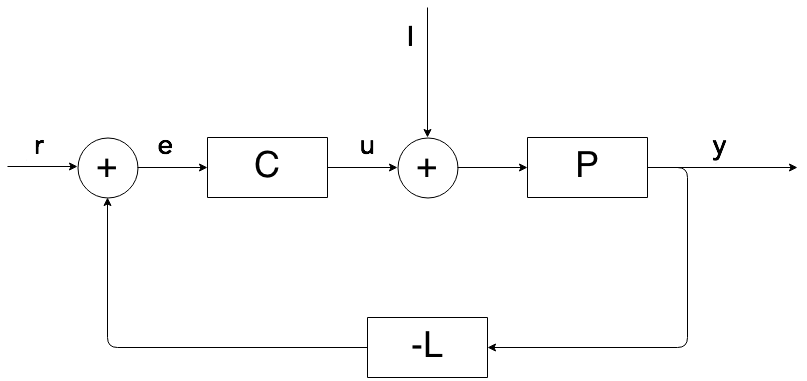
\includegraphics[width=0.8\textwidth]{process_one_regul.png}
    \caption{Single PID-regulator controlling process}
    \label{1}
\end{figure}

\subsection{The PID-controller}
The PID-controller is a very common controller. It can be separated in to three different parts as is seen in the formulae(FRaN FoRELaSNING 8):

\begin{equation}
   u(t) = K(e(t) + \frac{1}{T_i}\int\limits_0^t e(\tau) \mathrm{d}\tau + T_d\frac{\mathrm d e(t)}{\mathrm d t})
\end{equation}
\begin{equation}
   U(s) = KE(s) +  \frac{K}{sT_i}E(s) + KT_d s E(s)
\end{equation}
\begin{equation}
   U(s) = P +  I + D
\end{equation}

The term P is called the proportional term, and it calculates the control signal U depending of the size of the error $E = R - Y$ (where $R$ is the desired reference value and $Y$ the actual measured value). However, using only a $P$-controller could generate an undesirable stationary error. That is the reason to use the $I$-part which grows in case of an stationary error and thus minimising it. The $D$-part extends the regulator even more by introducing prediction and thus even more precise control.

To define the appropriate parameter values for the controller both analytic and empirical methods were used. Intitially, the controller used only the $P$ and $I$ parts. When stability was achieved for this configuration, the $D$-part was calibrated to give a smooth controlling of the Segway. To minimise impact of drift in the gyro sensor, a feed-forward loop was also introduced. The signal from the sensor is filtered through a low pass filter and then an offset is added to account for the increasing magnitude of the disturbance.



%FRÅN INFÖR
%The system will be controlled using a single PID-controller. Since the only measurable output is the angle offset to the horizontal plane, the system can be controlled with a single controller, this angle will serve as our reference. The controller will need to be very precise when controlling the system, which suggests that all three parts of the controller will have to be used. Additionally, the parameters of the different parts will have to be fine-tuned in order to achieve stability.
 %   Assuming that the sensor will output an analog signal, the controller has to be able to sample the signal to compute its control signal. Given the fact that a segway is very sensitive to errors, the controller will need to sample rather fast in order to keep the segway balanced at all times.

%To further stabilize the segway, state feedback will be used. This is to prevent the segway from falling due to slanting floors or dirt in its way. The segway should be able to balance regardless of where it is placed (within reasonable limits, of course).


  %Detta blir en underunderrubrik
\section{User Interface}

\subsection{Running the Segway}


The user uploads the program to the EV3 brick via Bluetooth. This is easily done through the leJOS-plugin for Eclipse, which uploads a jar-file that the leJOS system can use.
Once the program is running on the Segway, Telnet is used to communicate with the Segway. It is very easy to establish a connection via Telnet, the IP-address is found on screen of the EV3 brick. The working commands that can be run over Telnet are listed below.

\begin{itemize}
\item \textbf{start} - starts the controller, allowing the Segway to balance
\item \textbf{stop} - stops the controller, making the Segway stop balancing (and fall over)
\end{itemize}

\noindent Using the command \textbf{stop} will not terminate the controller thread, meaning the Segway can start again without having to restart the system and reconnecting using Telnet. In order to terminate the program, the user clicks the \"Stop Program\" button found in the leJOS GUI found in the leJOS Eclipse-plugin.

\subsection{Plotter}
  %Detta blir en underunderrubrik
  
\section{Implementation}
\subsection{Initial work}
The initial work consisted of getting familiar with the equipment. The first design was a tall and minimalistic Segway with big wheels. It was a temporary design, but necessary for a quick start. Right from the beginning it was clear that Java was the language that should implement the considered real-time system. The approach required a Java virtual machine on the Lego Mindstorm EV3. The most reliable solution to that problem was leJOS\footnote{\url{http://www.lejos.org/}} which is a firmware replacement for Lego Mindstorm, developed for precisely this approach. 
\\[3ex]
A lot of the initial software development derived from the laboratory assignment 1, where a ball and beam process\footnote{\url{http://www.control.lth.se/previouscourse/FRTN01/Lab1_15/Laboratory1.html}} was developed using a PID regulator. But alot of the initial work consisted of installing leJOS and establishing a bluetooth connection to the EV3 device. 
\\[3ex]
Quickly we aimed for our first milestone, making the Segway self-balancing. After research and discussion it was clear that the Segway needed a PI controller and a gyro sensor to achieve that. 

\subsection{Software design}

As stated above the initial skeleton was based on the "Ball and beam" process, which has a lot of similar design considerations as a segway. A Regul class and Opcom class is used in a similar way as in the laboratory.

The main structure of the programs controlling the segway consists of two different smaller program. One Segway program that runs on the LEGO Mindstorm EV3 brick that handles the control of the Segway and works as a server to enable connection from a Operator program. The other program is the Operator program that runs on a computer and is used for setting the reference- and parameter values to the Segway. It is also used to plot the signals from the LEGO gyroscope, the calculated control signal and the reference value in a window. Each program uses threads with shared resourses and thereby needs a safe way to share these. This is accomplished using monitors implemented using the Java keyword synchronized in both programs.


\subsubsection{Segway}
The program that runs on the Segway is stored in the package called hardware (see figure 1 for UML-diagram). It consists of a Main program that starts the controller thread (the \texttt{Regul} class) and the thread used for communication between the LEGO program and the Operator program called \texttt{CommunicationThread}. All shared data between the threads are stored in a class called \texttt{Monitor}, this class contains synchronized get- and set-methods for needed variables which enables the threads to share their data in a thread safe way. The controller is implemented in a class called \texttt{Regul} which is inspired by the design of the Regiulator used in the ´Ball and beam process`. \texttt{Regul} contains an instance of the class \texttt{Segway} which in its turn contains instances of the classes \texttt{SegwayMotor} and \texttt{GyroSensor} these classes contains methods to control the motors and read gyroscope values. Using the values from the gyrosensor regulator calculates the control values that is sent to the motors by using instances of the class \texttt{PID} which is an implementation of a PID-regulator. The controller both limits the signals and uses anti-windup for the I-part of the controller. It also contatins methods to change the parameter values of the Segway.


\subsubsection{Operator}
The Operator program (see figure 2 for UML-diagram)  contains a Main class that starts two threads. One, the CommunicationThread, reads the values of the signals from the Segway program and updates a monitor that contains the current values. PlotThread is used to read current signal values from the monitor and update the PlotOperatorGUI. There is two controller input GUI:s, ParameterGUI and ReferenceGUI that read the preferred reference value and parameters from the graphical interface and by using an actionhandler stores the new reference value in the monitor. The communication thread then reads the reference signal from the monitor and sends, if necessary, the new reference value to the Segway.

\subsection{Physical design and hardware}
Early on it was clear that the initial build of the Segway had a lot of flaws. The position of the actual EV3 brick didn't give the Segway equilibrium and there was no actual thought behind the design, besides making it tall for easier control. Tuning the PID parameters would not be an easy task with the present design. The solution was to rebuild it all, where stability and equilibrium was the main goal. After some research an advanced and robust design was found on line, lego's official {\it Gyro Boy}   implementation\footnote{\url{http://robotsquare.com/wp-content/uploads/2013/10/45544_gyroboy.pdf}}, where our design consists of the vital parts in the tutorial. The design process is well documented in the GitHub repository\footnote{\url{https://github.com/hilmers/LegoSegwayFRTN01}}. 
\\[3ex]
At this part the Segway was robust and well-balanced, but the {\it HiTechnic Gyro Sensor} introduced some issues. It was quickly discovered that the Gyro had a habit to cause drift. The drift affected the Segway's zero point position, in which it is self-balanced. The problem could partially be derived from the EV3 battery, lower battery levels lead to higher drift. But even with a fully-loaded or even plugged in battery there was a drift problem. By introducing a Low Pass Filter in the {\it Gyro Sensor} class the problem was minimised, but still present. Adding an empirically developed constant to the sampled value from the Low Pass Filter proved effective. The produced drift constant was divided by the amount of samples to give a relevant offset. Research on the Internet showed that this was a well known problem with the {\it HiTechnic gyroscopic Sensor} and a perfect solution was yet to be found. 
\\[3ex]
Accelerometer ....      

\subsection{Parameter tuning}
With a robust design and well implemented PID, the last piece of the puzzle are the PID parameters. As a start point we used parameters comparable to the ones used in the Ball and Beam process, and derived the work from that. Brute force tuning resulted  


\newpage
%Källförtecknhing
\bibliographystyle{unsrt}
\bibliography{bibliography.bib}

\end{document}                 % The input file ends with this command.
